In this section, we introduce our algorithm for natural language generation,
entitled ``Sentence Tree Realization using UCT" (STRUCT).  We begin
by describing how we formalize the problem as an MDP.  We then explain
the modifications we have made to UCT in order to improve
its applicability in NLG.  We discuss the inputs to STRUCT and explain
how those can be specified.  We present STRUCT's pseudocode, and describe
our method of creating reward functions for our MDPs.  Next, We detail enhancements
to STRUCT external to the MDP planning problem, and conclude by analyzing
STRUCT's benefits and weaknesses compared to other popular
NLG algorithms.

\section{NLG as planning in an MDP}
We formulate NLG as a planning problem on a Markov decision process
(MDP)  Using such an approach with a suitable defined MDP
(explained below) allows us to naturally handle
probabilistic grammars as well as formulate NLG as a planning problem,
unifying the distinct lines of attack described above. Further, the
strong theoretical guarantees of UCT translate into fast generation in
many cases, as we demonstrate in our experiments.
As the state space size in the language generation MDP is
very large, we use a variation of the UCT algorithm in our system,
described in chapter 2.2.

As discussed earlier, an MDP is made up of a set of states, a set of
actions, a transition function, a reward function, and a discount factor.
In our transformation of the NLG problem into an MDP, we must define
each of these in such a way that a plan in the MDP becomes a sentence
in a natural language.  Our set of states, therefore, will be partial
sentences.  Each partial sentence possible in the language defined by
the generation problem's grammar is a state in our MDP.  There are,
therefore, an infinite number of states, since TAG adjoins can be
repeated indefinitely.  Our set of actions will correspond to a single
TAG substitution or adjoin at a particular valid location in the tree.
Since we are using LTAGs in this work,
this corresponds to adding a single word to the partial sentence.
This definition makes our transition function intuitive; it is simply the
mapping between a partial sentence / action pair and the partial
sentence which results from the TAG adjoin / substitution.
Our reward function, intuitively, describes how close we are
to the goal semantic meaning.  The construction of this function
is nontrivial and will be described in detail later.  We use a
discount factor of 1; this is motivated by our willingness to tolerate
lengthy sentences in order to ensure we get a generated result
that matches our goal.

\section{Modifications to UCT}

We made three modifications to UCT in order to increase its usability
for NLG tasks.  This is motivated by the difference between normal
use of UCT and the NLG application's needs.
UCT is normally used to search for sparse rewards
in a tree of finite depth.  Our reward functions, which we will describe
later, provide feedback after every action, and our tree is of potentially
infinite depth.  Consequently, we have implemented a depth limit
on our tree search.  We perform a number of actions in the
default policy stage of UCT equal to a parameter $d$.  We then
evaluate our reward function at the state we reach and push that
reward up to the root as usual.

Second, UCT is normally used in an environment where the transition
function is nondeterministic.  UCT is often used in an adversarial environment,
like chess or Go, and consequently searches for the best average case
from a given state.  We do this because the original formulation
of UCT is designed to work in adversarial situations, in such cases,
selecting the absolute best may be risky if the opponent can respond
with something that can also lead to a very bad result. In our case,
however, there is no opponent, so we can freely choose the action
leading to best overall reward.

Third, UCT normally ends the tree policy phase by selecting an action
from the unexplored actions list randomly.  Since we can reasonably
expect that in the domain of NLG, there could easily be a better ordering
of those unexplored actions which can be known before selecting them.
For instance, some words might be substantially more common in
practice than others, so we should search trees which use those
words before other trees.  STRUCT allows for a heuristic to order the nodes
it searches.

Our choice of UCT is motivated by the high branching factor encountered in natural language generation when dealing with
large grammars as well as the belief that optimal sentences to accomplish a communicative goal are not required in most
discourse. In fact, generating optimal sentences may be more time-consuming than nearly-optimal plans which accomplish
the goal nearly as well.

\section{STRUCT}
\subsection{Inputs to STRUCT}

STRUCT takes four inputs and generates a single sentence.  These inputs are a grammar,
a lexicon, a worldfile, and a communicative goal.

A grammar, for our purposes, contains a set of trees, divided into two sets (initial and auxiliary).
These trees need to be annotated with the entities in them.  Entities are defined as any element
anchored by precisely one node in the tree which can appear in a proposition representing the
semantic content of the tree.  These trees are uniquely named, and also contain an
annotation (+) representing the lexicalized node.  See Appendix A for an example of a combined
grammar / lexicon.

The lexicon that we use is a list of permissible word-tree pairings, annotated with the meaning of
the pairing.  For instance, if the grammar contained a tree named "a.adj", (N (A+) (N-foot*))
(an adjoining tree for prepending an adjective to a noun, whose foot node is an entity named "foot"),
then the lexicon might contain an entry "a.adj: ['red', 'red(foot)]".  That would mean that the overall
LTAG that we are using contains the tree named "a.adj", lexicalized to 'red', and that when that tree
is applied to a sentence, the sentence's meaning is adjusted to include red(name of the foot node).
Appendix A contains an example of a combined grammar / lexicon.

A worldfile is a list of all statements which are true in the world surrounding our generation.
Matching entity names refer to the same entity.  Since we use the grounding assumption
to simplify our search, we need to include all statements which are true.

The communicative goal is just a list of propositions with dummy entity names.
These proposition names follow the same rules as those in worldfiles.
For instance, a communicative goal of 'red(d), dog(d)' would match a sentence 
with the semantic representation 'red(subj), dog(subj), cat(obj), chased(subj, obj)',
like "The red dog chased the cat", for instance.
As shown here, the communicative goal does not have to refer to any "central meaning" of the sentence as a human would select it, but rather
to propositions which the sentence affirms.  Appendix B contains an example of a communicative
goal and a number of sentences which satisfy it.

\subsection{The STRUCT Algorithm}
We now describe our approach, called Sentence Tree Realization with
UCT (STRUCT).
We begin with the state representing the empty tree.  The empty tree
contains no semantic meaning whatsoever, and is made up of a single
nonterminal, ``S".  Recall that the actions which can be taken from
every state are tree adjoin / tree substitution actions described in the
LTAG / PLTAG which defines the language we search over.
Since trees in LTAGs are associated
with individual words, actions can be interpreted as adding a specific
semantic meaning to the overall sentence while describing precisely
the syntactic environment in which these words can occur.
These adjoin operations can also
define arguments for the word in question.  For instance, the
location of the subject and object of a verb relative to the verb itself.
In this way, the tree shown in Figure \ref{s-to-npvp} defines the
``subject" and ``object" of the verb specified.
Further, since all recursive phenomena are
encoded in auxiliary trees, we factor recursion from the domain of
dependencies \cite{bauer2009statistical}, and can add auxiliary trees
to partial sentences without breaking dependency links between nodes.
In situations where the sentence is complete (no nonterminals without
children), we add a dummy action to stop generation and emit the
sentence.  Note that a complete sentence does not necessarily imply
a terminal state because adjoin operations can still be performed
(e.g. ``The dog ran'' could be expanded to ``The black dog ran quickly'').

In order to control the search space, we restrict the structure of the
MDP so that while substitutions are available, only those operations
are considered when determining the distribution over the next state,
without any adjoins.  This also allows us to generate a
complete and valid sentence quickly.  This allows STRUCT to operate as
an anytime algorithm, described further below.

From this point, we simply use our modified version of UCT as described
above to plan in the MDP from the initial state specified above.  See
Figure \ref{uct-code} for the general algorithm.

\begin{figure}[t]
\centering
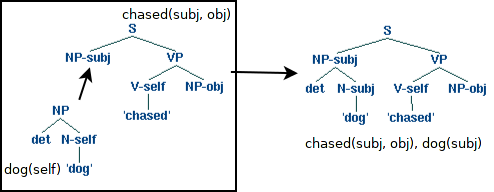
\includegraphics[width= 0.7 \linewidth]{sub-example.png}\label{examples-s}
\caption{An example tree substitution operation in STRUCT.}
\end{figure}

\begin{figure}[t]
\centering
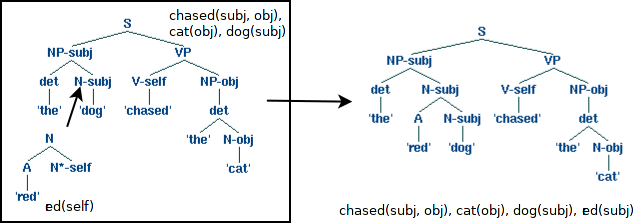
\includegraphics[width= 0.7 \linewidth]{adjoin-example.png}\label{examples-a}
\caption{An example tree adjoining operation in STRUCT.}
\end{figure}

\begin{figure}
\caption{The STRUCT Algorithm.}\label{uct-code}
\begin{algorithmic}[1]
\REQUIRE Number of simulations $numTrials$, Depth of lookahead $maxDepth$
\ENSURE Generated sentence tree
\STATE $bestSentence \gets$ nil
\WHILE {User has not interrupted generation}
\STATE $state \gets$ empty sentence tree
\WHILE{$state$ not terminal}
	\FOR{$numTrials$}
		\STATE $testState \gets state$
		\STATE $currentDepth \gets 0$
		\IF{$testState$ has unexplored actions}
			\STATE Apply one unexplored PLTAG production chosen
                        uniformly at random to $testState$
			\STATE $currentDepth$++
		\ENDIF
		\WHILE{$currentDepth < maxDepth$}
			\STATE Apply PLTAG production selected by tree
                        policy (Equation~\ref{eqn:uct})
			\STATE $currentDepth$++
		\ENDWHILE
		\STATE calculate reward for $testState$
		\STATE associate reward with first action taken
	\ENDFOR
	\STATE $state \gets$ maximum reward $testState$
	\IF{$state$ score $> bestSentence$ score \AND $state$ has no nonterminal leaf nodes}
		\STATE $bestSentence \gets state$
	\ENDIF
\ENDWHILE
\ENDWHILE
\RETURN $bestSentence$
\end{algorithmic}
\end{figure}

\section{Reward Function Definition}

 The reward function for a state must be defined exclusively in terms
 of the state in question.  The reward function serves as a metric to
 rank the favorableness of a sentence.  This reward function must be
 efficiently computable since it will be computed for every iteration
 in the UCT algorithm.  It must also be able to provide a value for a
 partial sentence since, due to the depth limit, a complete sentence
 may not always be reached.  There are, of course, many
possible reward functions which fulfill all of these requirements.

Since the reward function is specific to the individual generation
problem and guides the search for the correct meaning in the
given world, we designed a method for automatically constructing
a reward function from these inputs.
 
We found two reward functions which will
 return satisfactory results on a variety of experiments, but have complementary
properties where they differ.  The first reward function
 which we found to be useful considers a goal as well as a 
 grounded world.  It examines all possible mappings of entities present in
 a given sentence's annotation to entities present in the world, then returns
 a high value if there are any mappings which are both possible (contain no statements
 which are not present in the grounded world) and fulfill the goal (contain the
 goal statement).  This reward function happens to perform somewhat slowly since it includes
a subsumption problem as a step within it.  It runs in $O(N!)$ time, where
N is the number of entities present in the sentence.  The pseudocode for this algorithm
is present in \ref{struct-a}

\begin{figure}
\caption{The STRUCT$_a$ reward function.}\label{struct-a}
\begin{algorithmic}[1]
\REQUIRE State $s$, World $w$, Goal $g$
\ENSURE Numerical reward
\STATE $bestReward \gets$ -INF
\STATE $countValidPermutations \gets$ 0
\FOR {permutation $p$ of entities in the world}
	\STATE $currentReward \gets 0.0$
	\IF {all $prop$ in $s$, mutated by $p$, are in $w$}
		\STATE $currentReward \gets$ 10.0
		\STATE $countValidPermutations++$
	\ENDIF
	\IF {$g$ is satisfied by $s$ mutated by $p$}
		\STATE $currentReward += 50.0$
	\ENDIF
	\FOR {entity $e$ in $p$}
		\IF {$e$ is uniquely described by $s$, mutated by $p$}
			\STATE $currentReward += 1.0$
		\ENDIF
	\ENDFOR
	\IF {$currentReward > bestReward$}
		\STATE $bestReward \gets currentReward$
	\ENDIF
\ENDFOR
\IF {$countValidPermutations == 0$}
	\RETURN -INF
\ENDIF
\RETURN $bestReward / countValidPermutations$
\end{algorithmic}
\end{figure}

Of course, if we can remove the permutation from this algorithm,
we can get much better performance.  We know that in most cases,
STRUCT won't need to consider combinations of entity mapping and
can get by with simply considering whether an entity, by itself, could
satisfy the goal.  To this end, we present STRUCT$_b$, in Figure \ref{struct-b}.

\begin{figure}
\caption{The STRUCT$_b$ reward function.}\label{struct-b}
\begin{algorithmic}[1]
\REQUIRE State $s$, World $w$, Goal $g$
\ENSURE Numerical reward
\STATE $maxReward \gets 0$
\FOR {entity $e$ in the world}
	\STATE $currentReward \gets 0$
	\STATE $possibleEntities \gets 0$
	\FOR {proposition $p$ in $s$}
		\FOR {entity $e_p$ in $p$}
		\IF {$p$ could be true if $e$ is $e_p$}
			\STATE $possibleEntities++$
		\ENDIF
		\IF {$g$ could be true if $e$ is $e_p$}
			\STATE $currentReward += 5$
		\ENDIF
		\ENDFOR
	\ENDFOR
	\IF {$possibleEntities == 0$}
		\STATE $currentReward \gets -INF$
	\ELSE
		\STATE $currentReward = currentReward / possibleEntities$
	\ENDIF
	\IF {$currentReward > maxReward$}
		\STATE $maxReward = currentReward$
	\ENDIF
\ENDFOR
\RETURN $maxReward$
\end{algorithmic}
\end{figure}

Our experiments will show that STRUCT$_b$
has better performance than STRUCT$_a$, but that STRUCT$_a$ generates better
sentences in some domains.  This is due to the occasions on which
permutation considerations apply; for instance, we'll need those considerations
if we wish to generate sentences like ``The dog which chased the black cat ran
after the white cat," because we'll need to care about which cat the dog
chased and which it ran after.

\section{Enhancements External to the MDP}

The algorithm as described above performs well, but there are enhancements
external to UCT which can increase performance and provide additional
positive qualities.

\subsection{Execution as an Anytime Algorithm}
 With the MDP definition above, we use UCT to find a solution sentence
 (Figure~\ref{uct-code}). After every action is
 selected and applied, we check to see if we are in a state in which
 the algorithm could terminate (i.e. the sentence has no nonterminals
 yet to be expanded).  If so, we determine if this is the best
 possibly-terminal state we have seen so far.  If so, we store it, and
 continue the generation process. If we reach a state from which we
 cannot continue generating, we begin again from the start state of
 the MDP. Because of the structure restriction above (substitution
 before adjoin), STRUCT also generates a valid sentence quickly. These
 modifications enable STRUCT to perform as an anytime algorithm, which
 if interrupted will return the highest-value complete and valid
 sentence.

After this point, any time that there are no substitutions
available (all nonterminals have at least one child), we record the
current sentence and its associated reward.  Such a sentence is
guaranteed to be both grammatical and complete.  If generation is
interrupted, we return the highest-value complete and valid sentence.
In this way, our approach functions as an anytime algorithm.

We note that neither of these modifications cause any loss of
generality.  Our Anytime-UCT implementation will work on any suitably
defined MDP.  We implemented the system in Python 2.7.

 Clearly, the action set can get very large for a large grammar or for
 a long sentence with many locations for adjoining.  Still, this is the
 only way to ensure that we can generate all possible grammatical
 sentences.  UCT deals very well with this large action set due to the
 pruning inherent in its iterated Monte Carlo sampling method.  We can
 further compensate for this large action set by increasing the number
 of samples, if necessary.  It should also be noted that most
 combinations of these actions are order-independent; for instance, two
 actions, each adjoining an adjective to the subject and object of the
 sentence, respectively.  It is also notable that, occasionally, the
 order of some words in a sentence is not important.  ``A small white
 teapot'' and ``a white small teapot'' convey the same semantic
 information despite the different ordering of their adjectives.

\subsection{Grammar Pruning}

English is, of course, a very large language.  In most communicative goals, it is
not necessary to consider every one of the possible configurations of words and
meanings that make up the set of possible expressions.  If this was necessary,
it would be completely intractable to generate even the simplest sentences.

The approach that we took to reduce the complexity of generation is to ensure that
generation takes place using exclusively the relevant words.  This is done by selecting
the entities in the world which are needed for the goal, then iteratively selecting all
meanings transitively related to those entities.  Once we have selected all these meanings,
we will remove all words from the grammar which have a meaning not contained in this list.

In practice, this means that we often need a very small proportion of the overall language,
speeding generation significantly.\\

In the next section, we will perform an experimental evaluation of the
performance of STRUCT as compared to CRISP.